\documentclass[11pt,a4paper]{article}
\usepackage[utf8]{inputenc}
\usepackage[T1]{fontenc}
\usepackage{amsfonts}
\usepackage[french]{babel}
\frenchbsetup{StandardLists=true} % à inclure si on utilise \usepackage[francais]{babel}
\usepackage{enumitem}
\usepackage{amssymb}
\usepackage{amsmath}
\usepackage[left=2cm,right=2cm,top=2cm,bottom=2cm]{geometry}
\usepackage{multirow}
\usepackage[dvipsnames]{xcolor}

\usepackage[T1]{fontenc}
\usepackage{graphicx}

\usepackage{setspace}
\singlespacing

\usepackage{pstricks}
\usepackage{xkeyval}
\usepackage{pst-labo}


\usepackage{multicol}
\usepackage{caption}
\usepackage{fancyhdr}
\pagestyle{fancy}
\renewcommand\headrulewidth{1pt}
\fancyhead[L]{Lycée Denis Diderot }
\fancyhead[R]{Classe de Première}
\setcounter{page}{3}\fancyfoot[C]{page \thepage}
\fancyfoot[R]{Année 2024-2025}
\fancyfoot[L]{Alexis RUIZ}
\usepackage{multirow,tabularx,booktabs}
\usepackage[tikz]{bclogo} 
\usepackage{circuitikz}

\newcommand{\cadreblanc}[1]{%
\medskip\framebox[\linewidth][c]{%
\rule{0mm}{#1mm}}\par
\medskip}

\usepackage{awesomebox}
\setlength{\aweboxvskip}{0mm}
\usepackage{pifont}
\usepackage{chemmacros}
\chemsetup{modules=all}
\setlength{\columnseprule}{.25mm}

\renewcommand{\arraystretch}{2}
\newcommand*\acocher{\quitvmode{\fboxsep0pt \fboxrule0.8pt \fbox{\vrule height1.8ex depth.1ex width0pt \vrule height0pt depth0pt width1.9ex }}}

\newcolumntype{C}[1]{>{\centering\arraybackslash }b{#1}}

\newcommand{\code}{\awesomebox[black]{2pt}{

\includegraphics[scale=0.15]{../Chapitre 1 - Energie et puissance électrique/images/frame.png}
}{black}}

\newcommand{\moteur}{\awesomebox[black]{2pt}{

\includegraphics[scale=1]{images/moteur.jpg} 
}{black}}

\newcommand{\defbox}{\awesomebox[black]{2pt}{
\includegraphics[scale=0.5]{../Chapitre 1 - Energie et puissance électrique/images/appel exam.png}}{black}}

\newcommand{\defconclusion}{\awesomebox[black]{2pt}{\rotatebox{90}{\Large{\textbf{Conclusion}}}}{black}}

  \newenvironment{itemize*}%  % listes compactes
    {\begin{itemize}%
      \setlength{\itemsep}{0pt}%
      \setlength{\parskip}{0pt}}%
    {\end{itemize}}

\frenchbsetup{StandardLists=true}



\begin{document}


\flushleft \textbf{NOM : \hfill Classe : \hspace{3cm} ~~\\[2mm]
Prénom:\\[0,4cm]
}
\hrule\
\\[0,2cm]

\begin{center}
 \LARGE{TP1 - Quelle est la tension en sortie d'un transformateur ? }
\end{center}

\vspace{3 mm}

\normalsize

\hrule\
\\[0,2cm]
   \begin{center}
   \textbf{Le soin et la rédaction interviendront dans la notation.}
   \end{center} 

\vfill 



\fcolorbox{black}{white}{\textbf{1. Expérience}}  \\

 \begin{enumerate}[label*=1.\arabic*.]
 

     \item Réaliser le montage ci-dessous : 

     
\noindent%
\begin{minipage}{.4\textwidth}%
 \begin{bclogo}[couleur=white ,  arrondi =0.1 , logo = \bcinfo, epBarre =2]{ Matériel }

\begin{itemize*}
    \item 1 générateur 12V CA
    \item 1 transformateur
    \item 1 oscilloscope
    \item 6 fils de connexion
\end{itemize*}
\end{bclogo}

\end{minipage}%
\hfill
\begin{minipage}{.5\textwidth}%
\begin{center}
    
\begin{circuitikz}
\draw (0,0)node[transformer core, yscale=1.25] (T) {}; %placement du transformateur
\draw (T.A2) --++(-1,0) to [sV] ($(T.A1)+(-1,0)$) -- (T.A1); %connexion partant de l’ancr
%\draw (T.A2) node[below]{T.A2}; %placement du nom de l’ancre A2 : T.A2
%\draw (T.A1) node[above]{T.A1}; %placement du nom de l’ancre A1 : T.A1
\draw(T.B2) to [short, o-] (3.5,-1.3) node[eground]{};
\draw(T.B1) to [short, o-] (3.5,1.3) [->] node[right]{Y2};
\draw(-2,1.3) to [short, o-] (-3,1.3) [->] node[left]{Y1};
%\draw(T.B2) to (-o) node[behind]{Borne noire};
\draw(-2,-1.3) to [short, o-]  (-3,-1.3)  node[eground]{};
\draw (2.5,1.3) to[oscope] (2.5,-1.3);
\node[text width=1cm] at (1.5,-2.1) {Borne Noire};
\node[text width=1cm] at (1.5,2.1) {Borne m=1};

\end{circuitikz}



\end{center}
\end{minipage}%

\vfill 
    
\defbox{\fbox{
\begin{minipage}{8cm}{

Appeler M Ruiz pour qu'il vérifie le montage.}

\end{minipage}
}}

\vfill

\item Reproduire l'écran de l'oscilloscope et compléter les tableaux en relevant les valeurs. 
\noindent%
\begin{minipage}{.45\textwidth}%

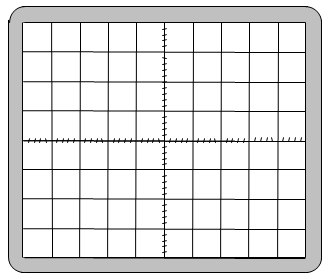
\includegraphics[scale=0.6]{images/ecran oscillo.png} 

\end{minipage}%
\hfill
\begin{minipage}{.45\textwidth}%

Tension~d'~entrée (Y1) 

\renewcommand{\arraystretch}{2.8}
\begin{tabularx}{8 cm}{|c||X|X|}
\hline
Valeurs & $U_{1~Max}=$ & $T_1=$\\
\hline 
\end{tabularx}

\vspace{1mm}

\renewcommand{\arraystretch}{2.8}
\begin{tabularx}{8 cm}{|c||X|X|}
\hline
Calculs & $U_{1~Eff}=$ & $f_1=$\\
\hline 
\end{tabularx}

\vspace{5mm}

Tension de sortie (Y2)

\renewcommand{\arraystretch}{2.8}
\begin{tabularx}{8 cm}{|c||X|X|}
\hline
Valeurs & $U_{2~Max}=$ & $T_2=$\\
\hline 
\end{tabularx}

\renewcommand{\arraystretch}{2.8}
\begin{tabularx}{8 cm}{|c||X|X|}
\hline
Calculs & $U_{2~Eff}=$ & $f_2=$\\
\hline 
\end{tabularx}

\end{minipage}%

\vfill 

\item Comparer les valeurs de $U_{Eff}$ et de $f$ en entrée et en sortie. 

\vspace{8mm}
\dotfill 

\vfill 

\newpage 

\item Reproduire l'écran de l'oscilloscope et effectuer les mêmes mesures en branchant l'oscilloscope à la borne m = 0,5 du transformateur. 

\noindent%
\begin{minipage}{.45\textwidth}%

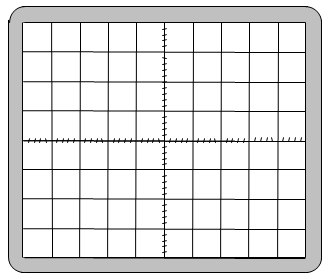
\includegraphics[scale=0.6]{images/ecran oscillo.png} 

\end{minipage}%
\hfill
\begin{minipage}{.45\textwidth}%

Tension~d'~entrée (Y1) 

\renewcommand{\arraystretch}{2.8}
\begin{tabularx}{8 cm}{|c||X|X|}
\hline
Valeurs & $U_{1~Max}=$ & $T_1=$\\
\hline 
\end{tabularx}

\vspace{1mm}

\renewcommand{\arraystretch}{2.8}
\begin{tabularx}{8 cm}{|c||X|X|}
\hline
Calculs & $U_{1~Eff}=$ & $f_1=$\\
\hline 
\end{tabularx}

\vspace{5mm}

Tension de sortie (Y2)

\renewcommand{\arraystretch}{2.8}
\begin{tabularx}{8 cm}{|c||X|X|}
\hline
Valeurs & $U_{2~Max}=$ & $T_2=$\\
\hline 
\end{tabularx}

\renewcommand{\arraystretch}{2.8}
\begin{tabularx}{8 cm}{|c||X|X|}
\hline
Calculs & $U_{2~Eff}=$ & $f_2=$\\
\hline 
\end{tabularx}

\end{minipage}%

\end{enumerate}

\vfill 

\fcolorbox{black}{white}{\textbf{2. Interprétation}}  \\

 \begin{enumerate}[label*=2.\arabic*.]

\item Calculer le rapport $\dfrac{U_{2~Eff}}{U_{1~Eff}}$ et comparer celui ci à la valeur de \textbf{m} en sortie du transformateur.  

\vspace{2mm}
\cadreblanc{15}

\vfill

\item Comparer les valeur des fréquences $f_1$ et $f_2$. 

\vspace{8mm}
\dotfill 
\end{enumerate}

\vfill 
\fcolorbox{black}{white}{\textbf{3. Validation}}  \\

Un transformateur est considéré comme "parfait" si $\dfrac{U_{2~Eff}}{U_{1~Eff}} = m $ avec moins de 1\% de différence. Vérifiez si votre transformateur est "parfait".

\cadreblanc{25}

\vfill 

\fcolorbox{black}{white}{\textbf{4. Conclusion}}  \\[2mm]

Quelle est le rôle du transformateur ? 

\cadreblanc{20}


\vfill 
\end{document}